\documentclass[a4paper,11pt]{article}

% Identificação
\newcommand{\pbtitulo}{MongoDB com Java e Python}
\newcommand{\pbversao}{1.1}

\usepackage{../sty/tutorial}

%----------------------------------------------------------------------
% Início do Documento
%----------------------------------------------------------------------
\begin{document}
	
\maketitle % mostrar o título
\thispagestyle{fancy} % habilitar o cabeçalho/rodapé das páginas

%----------------------------------------------------------------------
% RESUMO DO ARTIGO
%----------------------------------------------------------------------
	
\begin{abstract}
  % O primeiro caractere deve vir com \initial{}
\initial{A}\textbf{tualmente muito se tem comentado sobre bancos de dados não relacionais, também chamados de NoSQL. O conhecimento destes podem abrir várias portas e deve ser considerado um fator de extrema importância para garantir uma boa empregabilidade. É sempre importante estar atento a novas tecnologias e como elas resolvem problemas provenientes das limitações existentes no caso deste tipo de banco enormes quantidade de dados. Neste tutorial veremos o que vem a ser o banco MongoDB \cite{mongooficial} e como proceder sua utilização utilizando como pano de fundo a linguagem de programação Java \cite{javaoficial} e Python \cite{pythonoficial}.}
\end{abstract}

%-----------------------------------------------------------------------------
% CONTEÚDO DO ARTIGO
%-----------------------------------------------------------------------------

\section{Parte inicial}
MongoDB (de ``humongous'' - monstruoso) é um Sistema de Banco de dados não relacional, Orientado a Documentos e de fonte aberto. É parte da família de sistemas de Banco de Dados denominados \textbf{NoSQL}, ou seja, em vez de armazenar dados em tabelas - como é feito em um banco de dados relacional - armazena seus dados em uma estrutura como JSON, ou seja, documentos com esquemas dinâmicos. Este formato é conhecido como \textbf{JSON Binário} ou simplesmente BSON.
\begin{figure}[H]
	\centering
	
\includegraphics[width=0.5\textwidth]{imagens/logo.jpg}
	\caption{Logo do MongoDB}
\end{figure}

Possui como objetivo principal promover uma integração mais fácil e rápida com os dados. E possui as seguintes características:
\begin{itemize}[nolistsep]
  \item Escrito em linguagem de programação C++
  \item Gerenciar coleções de documentos BSON formato de intercâmbio de dados usado principalmente como um formato de armazenamento de dados e transferência de rede no banco de dados MongoDB.
  \item BSON é uma forma binária para a representação de estruturas de dados simples e matrizes associativas (chamados de objetos ou documentos no MongoDB)
\end{itemize}

\subsection{Criar o contêiner Docker}
A forma mais simples de termos o MongoDB é através de um contêiner no Docker, assim facilmente podemos ter várias versões do banco instalada e controlar mais facilmente qual banco está ativo ou não. E ainda colhemos o benefício adicional de não termos absolutamente nada deixando sujeira em nosso sistema operacional ou áreas de memória.

Baixar a imagem oficial: \\
{\ttfamily\$ docker pull mongo}

Criar uma instância do banco em um contêiner: \\
{\ttfamily\$ docker run --name meu-mongo -p 27017:27017 -d mongo}

Acessar o Shell de comandos do MongoDB no contêiner: \\
{\ttfamily\$ docker exec -it meu-mongo mongo admin}
\begin{lstlisting}
> show dbs
> use local
> show collections
> exit
\end{lstlisting}

Para encerrar o contêiner: \\
{\ttfamily\$ docker stop meu-mongo} 

Para iniciar novamente o contêiner: \\
{\ttfamily\$ docker start meu-mongo} 

\subsection{Shell - a console de comandos}
O Mongo Shell, também conhecida como Console de Comandos, utiliza uma interatividade entre comandos JavaScript e o MongoDB. Aqui é possível realizar operações administrativas como consultas ou manutenções de dados.

Mostrar as bases de dados existentes: \\
{\ttfamily> show dbs}

Criar (ou mudar) a base de dados para a atual: \\
{\ttfamily> use nome\_base}

Mostrar as coleções existentes na base de dados atual: \\
{\ttfamily> show collections}

Inserir (ou alterar caso o objeto tenha sido chamado anteriormente) um documento em uma coleção (se a coleção não existe será criada) na base de dados corrente (db é uma variável interna apontada para a base de dados atual) \\
{\ttfamily> db.nome\_colecao.save({campo1:valor1, ..., campoN:valorN})} 

Listar os documentos de uma coleção existente na base de dados atual: \\
{\ttfamily> db.nome\_colecao.find()}

Eliminar documento(s) de uma coleção existente na base de dados atual: \\
{\ttfamily> db.nome\_colecao.remove({campo:valor})}

Apagar uma coleção existente na base de dados atual: \\
{\ttfamily> db.nome\_colecao.drop()}

Apagar a base de dados atual: \\
{\ttfamily> db.dropDatabase()}

Se percebemos bem a única diferença do MongoDB para bancos relacionais é entendermos como é o relacionamento entre os objetos:
\begin{figure}[H]
	\centering
	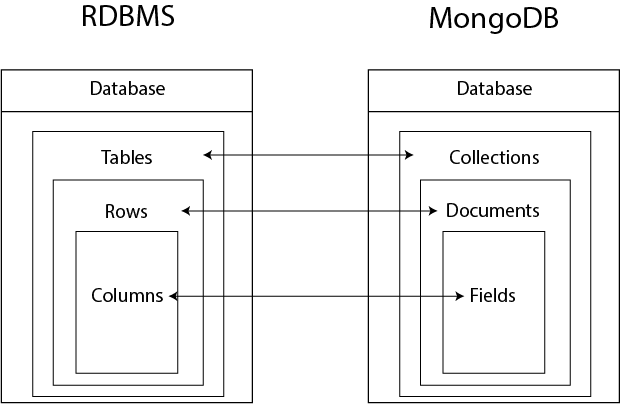
\includegraphics[width=0.5\textwidth]{imagens/comparativo.png}
	\caption{Comparativo entre os objetos do MongoDB e SQL}
\end{figure}

Para conhecer mais comandos do Shell, podemos acessar o seguinte endereço:  \url{https://docs.mongodb.org/manual/mongo/}

\section{Linguagem Java}
Java é considerada a linguagem de programação orientada a objetos mais utilizada no Mundo, ela é a base para construção de ferramentas como Hadoop, Pentaho, Weka e muitos outros utilizados comercialmente. Foi desenvolvida na década de 90 por uma equipe de programadores chefiada por \textit{James Gosling} para o projeto Green, na empresa Sun Microsystems - tornou-se nessa época como a linguagem que os programadores mais baixaram e o sucesso foi instantâneo. Em 2008 o Java foi adquirido pela empresa Oracle Corporation.

\subsection{Driver JDBC de Conexão}
Para proceder a conexão com Java, é necessário baixar um driver JDBC (Java Database Connection). Existem vários drivers construídos, porém o driver oficialmente suportado pelo MongoDB se encontra no endereço: \url{http://mongodb.github.io/mongo-java-driver}

Para utilizar o driver é necessário criar um projeto (vamos usar o \textbf{Spring Tool Suite 4}, utilize se quiser qualquer outro editor de sua preferência).

No STS4 acessar a seguinte opção no menu: File $\triangleright$ New $\triangleright$ Java Project. Informar o nome do projeto, não esquecer de modificar a opção "Use an environment JRE" para a versão correta da Java Runtime desejada e pressionar o botão Finish. Se está tudo correto teremos a seguinte situação na aba \textit{Project Explorer}:
\begin{figure}[H]
	\centering
	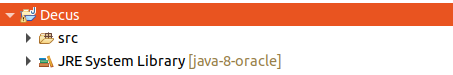
\includegraphics[width=0.5\textwidth]{imagens/projetoCriado.png}
	\caption{Projeto Decus criado}
\end{figure}

Vamos convertê-lo para um projeto Apache Maven. Clicar com o botão direito do mouse no projeto e acessar a opção: Configure $\triangleright$ Convert to Maven Project. Na janela apenas pressione o botão \textit{Finish}. Se tudo está correto observamos que o projeto ganhou uma letra \textbf{M} o que indica agora é um projeto padrão Maven. Então foi criado um arquivo chamado \textbf{pom.xml}. 

Acessar este arquivo e antes da tag BUILD, inserir a tag DEPENDENCIES:
\begin{lstlisting}
<dependencies>
  <!-- Logging -->
  <dependency>
    <groupId>org.slf4j</groupId>
    <artifactId>slf4j-simple</artifactId>
    <version>1.7.5</version>
  </dependency>
  <dependency>
    <groupId>org.slf4j</groupId>
    <artifactId>slf4j-log4j12</artifactId>
    <version>1.7.5</version>
  </dependency>
  <dependency>
    <groupId>org.slf4j</groupId>
    <artifactId>slf4j-api</artifactId>
    <version>1.7.5</version>
  </dependency>

  <!-- Driver Banco MongoDB -->
  <dependency>
    <groupId>org.mongodb</groupId>
    <artifactId>mongodb-driver-sync</artifactId>
    <version>4.0.4</version>
  </dependency>
</dependencies>
\end{lstlisting}

Agora a situação do projeto é esta:
\begin{figure}[H]
	\centering
	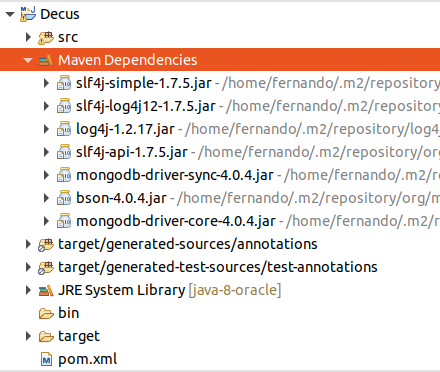
\includegraphics[width=0.6\textwidth]{imagens/dependenciasMaven.png}
	\caption{Dependências do Maven}
\end{figure}

Observamos que na pasta \textbf{Maven Dependencias} foi baixado a versão 4.0.4 do driver MongoDB.

\subsection{Testar a Conexão}
Estamos prontos para testarmos a conexão entre o MongoDB e o Java. Vamos criar um pequeno exemplo que servirá como teste, criar uma classe chamada \textbf{Escola} no pacote \textbf{decus.com} e inserir nesta a seguinte codificação:
\begin{lstlisting}
package decus.com;

import org.bson.Document;

import com.mongodb.client.MongoClients;
import com.mongodb.client.MongoClient;

import com.mongodb.client.MongoDatabase;
import com.mongodb.client.MongoCollection;
import com.mongodb.client.MongoCursor;

public class Escola {

  private MongoDatabase db;
  private MongoClient mongo;
  private MongoCollection<Document> col;

  protected MongoDatabase getDb() {
    return db;
  }

  protected MongoCollection<Document> getCol() {
    return col;
  }

  protected MongoClient getMongo() {
    return mongo;
  }

  protected boolean conectar() {
    try {
      mongo = MongoClients.create("mongodb://localhost:27017");
      db = mongo.getDatabase("escola");
      col = db.getCollection("aluno");
    } catch (Exception e) {
      return false;
    }
    return true;
  }

  protected boolean desconectar() {
    try {
      mongo.close();
    } catch (Exception e) {
      return false;
    }
    return true;
  }

  private void executar() {
    if (this.conectar()) {
      // Inserir os alunos
      Document doc = new Document("nome", "Mario da Silva").append("nota", (int)(Math.random() * 10));
      col.insertOne(doc);
      doc = new Document("nome", "Aline Moraes").append("nota", (int)(Math.random() * 10));
      col.insertOne(doc);
      doc = new Document("nome", "Soraya Gomes").append("nota", (int) (Math.random() * 10));
      col.insertOne(doc);

      // Listar os Alunos
      MongoCursor<Document> cursor = col.find().iterator();
      while (cursor.hasNext()) {
        doc = cursor.next();
        System.out.println(doc.get("nome") + ": " + doc.get("nota"));
      }
      cursor.close();
      this.desconectar();
    }
  }

  public static void main(String[] args) {
    new Empresa().executar();
  }
}
\end{lstlisting}

Esta classe adiciona três registros ao banco de dados contendo o nome do aluno e sua nota que é gerada de forma randômica e em seguida procede uma consulta para verificar se os registros foram realmente inseridos. A conexão e a desconexão ao MongoDB foi colocada em métodos separados.

No Shell utilizar os seguintes comandos para verificar os dados:
\begin{lstlisting}
> show dbs
> use escola
> show collections
> db.aluno.find()
\end{lstlisting}

E se tudo está OK, teremos o seguinte resultado:
\begin{figure}[H]
	\centering
	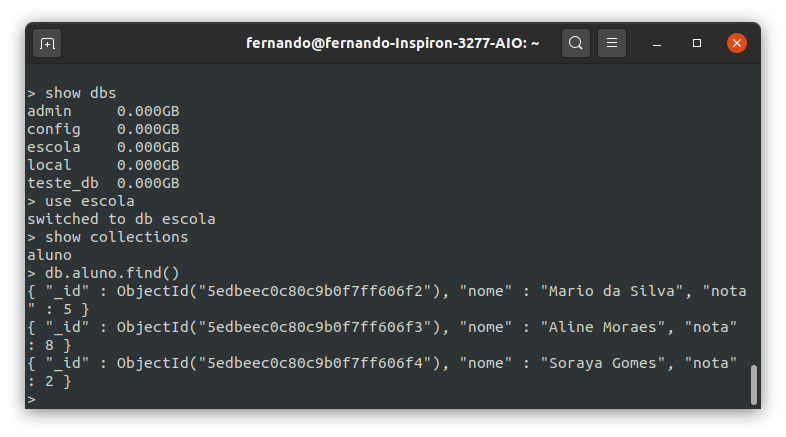
\includegraphics[width=0.5\textwidth]{imagens/testeOK.png}
	\caption{Execução do Shell}
\end{figure}

\subsection{Programação Java usando o MongoDB}
Nesta seção será visto como via linguagem Java é possível gerenciar os objetos do MongoDB. Os comandos dos exemplos a seguir foram escritos a partir dos objetos existentes no código anterior. Por esse motivo deixamos os métodos protegidos ao invés de particulares e criamos os tipo \textit{GET} para objetos que estão na mesma classe.

Criar uma nova classe chamada \textbf{TstComando}, que estende a classe \textbf{Escola} no mesmo pacote com a seguinte codificação:
\begin{lstlisting}
package decus.com;

public class TstComando extends Escola {

  public static void main(String[] args) {
    new TstComando().executar();
  }

  private void executar() {
    if (conectar()) {

      // Inserir o comando aqui

      desconectar();
    }
  }
}
\end{lstlisting}

Esta classe agora será a nossa principal, sendo assim removemos os métodos \textbf{main} e \textbf{executar} da classe \textbf{Escola} que já serviram a seu propósito. Lembre-se que a Programação Orientada a Objetos é uma metodologia e não uma linguagem, se pratica essa forma ao usarmos os princípios da Orientação a Objetos e aproveitar a qualidade de extensibilidade do código.

\subsection{Informações dos Objetos}
Para obter informações dos os objetos do MongoDB através do Java, é possível utilizar diversas ações. 

Listar as bases de dados existentes: \\
{\ttfamily for (String s: getMongo().listDatabaseNames()) \{ \\
\phantom{x}\hspace{4pt} System.out.println(s); \\
\} }

Criar um novo objeto na base de dados pelo seu nome: \\
{\ttfamily MongoDatabase db2 = getMongo().getDatabase("escola");}

Verificar quais são as coleções existentes em uma determinada base de dados: \\
{\ttfamily for (String s: getDb().listCollectionNames()) \{ \\
\phantom{x}\hspace{4pt} System.out.println(s); \\
\}}

Criar um novo objeto de coleção pelo seu nome e através deste obter a quantidade de registros existentes: \\
{\ttfamily MongoCollection<Document> col2 = getDb().getCollection("aluno"); \\
System.out.println("Total de Documentos:" + col2.countDocuments());}

Obter, em formato JSON (\textit{JavaScript Object Notation}), as coleções de uma determinada base de dados: \\
{\ttfamily ListCollectionsIterable<Document> it = getDb().listCollections(); \\
MongoCursor<Document> cursor = it.iterator(); \\
while (cursor.hasNext()) \{ \\
\phantom{x}\hspace{4pt} System.out.println(cursor.next().toJson()); \\
\} \\
cursor.close();}

Criar um índice para uma coleção, o parâmetro com valor igual a 1 informa que deve ser ordenado de forma ascendente, para descendente utilizar o valor -1: \\
{\ttfamily getCol().createIndex(new Document("nota", 1));}

Obter, em formato JSON, os índices de uma determinada coleção: \\
{\ttfamily ListIndexesIterable<Document> it = getCol().listIndexes(); \\
MongoCursor<Document> cursor = it.iterator(); \\
while (cursor.hasNext()) \{ \\
\phantom{x}\hspace{4pt} System.out.println(cursor.next().toJson()); \\
\} \\
cursor.close();}

Eliminar um indice de uma coleção: \\
{\ttfamily getCol().dropIndex(new Document("nota", 1));}

Obter, em formato JSON, os registros de uma determinada coleção: \\
{\ttfamily MongoCursor<Document> cursor = getCol().find().iterator(); \\
while (cursor.hasNext()) \{ \\
\phantom{x}\hspace{4pt} System.out.println(cursor.next().toJson()); \\
\} \\
cursor.close();}

Para os próximos exemplo, consideraremos o método executar() conforme o código abaixo e procedemos a inserção do comando descrito na posição indicada:
\begin{lstlisting}
private void executar() {
  if (conectar()) {

    // Inserir o comando aqui
    
    while (cursor.hasNext()) {
      System.out.println(cursor.next().toJson());
    }
    cursor.close();  
    desconectar();
  }
}
\end{lstlisting}

\subsection{Filtrar Coleções}
Limitar a quantidade de registros retornados (por exemplo 2 registros): \\
{\ttfamily MongoCursor<Document> cursor = getCol().find().limit(2).iterator();}

Trazer os alunos que obtiveram nota 10: \\
{\ttfamily MongoCursor<Document> cursor = getCol().find(new Document("nota", 10)).iterator();}

Através da classe \texttt{com.mongodb.client.model.Filters} é possível realizar a mesma ação: \\
{\ttfamily MongoCursor<Document> cursor = getCol().find(Filters.eq("nota", 10)).iterator();}

E com a utilização dessa classe, é possível realizar as seguintes ações:
\begin{itemize}[nolistsep]
  \item \textbf{Filters.ne} - registros não iguais a um determinado valor
  \item \textbf{Filters.gt} - registros maiores que um determinado valor
  \item \textbf{Filters.gte} - registros maiores ou iguais a um determinado valor
  \item \textbf{Filters.lt} - registros menores que um determinado valor
  \item \textbf{Filters.lte} - registros menores ou iguais a um determinado valor
\end{itemize}

Podemos utilizar as variáveis: \$eq (igual), \$ne (não igual), \$gt (maior), \$gte (maior ou igual), \$lt (menor) ou \$lte (menor ou igual). Obter todos os documentos da coleção com a nota é maior que 6: \\
{\ttfamily MongoCursor<Document> cursor = getCol().find( \\
	new Document("nota", new  Document("\$gt",6))).iterator(); } 

Parece mais complicado, porém é possível criar separadamente um objeto Documento e a partir dele compor combinações. Obter todos os documentos cujas notas são maiores que 3 e menores que 9: \\
{\ttfamily Document doc = new Document(); \\
doc.append("nota", new Document("$gt", 3).append("$lt", 9)); \\
MongoCursor<Document> cursor = getCol().find(doc).iterator();}

Para realizar a mesma consulta com a utilização dos filtros: \\
{\ttfamily MongoCursor<Document> cursor = getCol().find( \\
	Filters.and(Filters.gt("nota", 3), Filters.lt("nota", 9))).iterator();}

\subsection{Ordenações}
Através da classe \texttt{com.mongodb.client.model.Sorters}, e podemos utilizar as variáveis ``ascending'' e ``descending'' para obter ordenações: \\
{\ttfamily MongoCursor<Document> cursor = \\
	col.find().sort(Sorts.ascending("nota")).iterator();}

\section{Modificar dados da Coleção via Java}
Uma vez identificado o(s) documento(s) desejado(s) é possível proceder:
\begin{itemize}[nolistsep]
  \item Alterações. Utilizar os métodos updateOne ou updateMany.
  \item Eliminações. Utilizar os métodos deleteOne ou deleteMany.
\end{itemize}

Modificar a nota do aluno ``Mario da Silva'' para 5: \\
{\ttfamily getCol().updateOne(new Document("nome","Mario da Silva"), \\
	new Document("\$set", new Document("nota", 5))); }

Para eliminar o aluno ``Mario da Silva'': \\
{\ttfamily getCol().deleteMany(new Document("nome","Mario da Silva"));}

\subsection{Eliminar os Objetos}
Para eliminar a coleção ``aluno'': \\
{\ttfamily getCol().drop(); }

Para eliminar a base de dados ``escola'': \\
{\ttfamily getDb.drop();}

\section{Python}
Python é uma linguagem de programação de alto nível, interpretada a partir de um script, Orientada a Objetos e de tipagem dinâmica. Foi lançada por Guido van Rossum em 1991. Não pretendo nesta apostila COMPARAR essa linguagem com Java (espero que nunca o faça), fica claro que os comandos são bem mais fáceis porém essas linguagens possuem diferentes propósitos.

Todos os comandos descritos abaixo foi utilizado no JupyterLab \cite{jupyteroficial}, então basta abrir um Notebook e digitá-los em cada célula conforme se apresentam.

\subsection{Proceder a Conexão}
Baixar o pacote necessário: \\
{\ttfamily !pip install pymongo}

Importar os pacotes necessários: \\
{\ttfamily from pymongo import MongoClient \\
	import random}

Neste caso estamos utilizando o pacote \textbf{random} somente para criarmos o mesmo exemplo já visto e escolher uma nota aleatória para casa aluno.

Podemos nos conectar ao servidor de dois modos diferentes, desta forma: \\
{\ttfamily cliente = MongoClient('localhost', 27017)}

Ou desta forma: \\
{\ttfamily cliente = MongoClient('mongodb://localhost:27017/')}

Do mesmo modo também podemos nos conectar a base de dados de dois modos diferentes, desta forma: \\
{\ttfamily db = cliente.escola}

Ou desta forma: \\
{\ttfamily db = cliente['escola']}

Bem como a coleção de dois modos diferentes, desta forma: \\
{\ttfamily col = db.aluno}

Ou desta forma: \\
{\ttfamily col = db['aluno']}

\subsection{Inserir registros}
Inserir um único registro é uma questão de criar um dicionário e enviá-lo para a coleção: \\
{\ttfamily mario = \{ "nome": "Mario da Silva", "nota": random.randint(1,11) \} \\
col.insert\_one(mario) }

Inserir vários registros é necessário criar uma lista de dicionários e enviar a lista para a coleção: \\
{\ttfamily alunos = [ \\
\phantom{x}\hspace{4pt} \{ "nome": "Aline Moraes", "nota": random.randint(1,11) \}, \\
\phantom{x}\hspace{4pt} \{ "nome": "Soraya Gomes", "nota": random.randint(1,11) \} \\
] \\
col.insert\_many(alunos)
}

\subsection{Buscar registros}
Listar toda a coleção: \\
{\ttfamily for doc in col.find({}): \\
\phantom{x}\hspace{4pt} print(doc)}

Contar quantos registros tem na coleção: \\
{\ttfamily col.count\_documents({})}

Trazer o primeiro registro: \\
{\ttfamily col.find\_one()}

Trazer um determinado registro: \\
{\ttfamily col.find\_one(\{"nome": "Aline Moraes"\})}

Trazer determinados registros: \\
{\ttfamily for doc in col.find(\{"nota": \{"\$gt": 5, "\$lt": 7\}\}): \\
\phantom{x}\hspace{4pt} print(doc)}

\subsection{Atualizar registros}
Alterar determinado registro: \\
{\ttfamily col.update\_one(\{"nome": "Mario da Silva"\}, \{"\$set": \{"nota": 8\}\})}

Alterar um conjunto determinado de registros: \\
{\ttfamily col.update\_many(\{'nota': \{'\$lt': 5\}\}, \{'\$set': \{'nota': 4\}\})}

Eliminar determinado registro: \\
{\ttfamily col.delete\_one(\{"nome": "Mario da Silva"\}, \{"\$set": \{"nota": 8\}\})}

Eliminar um conjunto determinado de registros: \\
{\ttfamily col.delete\_many(\{'nota': \{'\$lt': 5\}\}, \{'\$set': \{'nota': 4\}\})}

\section{Conclusão}
Penso que depois dessa apostila, será possível usar todo o poder do banco MongoDB para seus trabalhos, pois como vimos é bem fácil realizar os passos nesse banco pouco importa a linguagem de programação. Não busquei nesta mostrar um exemplo mais completo para não limitar suas pesquisas e devemos considerar esta apenas como um pontapé inicial (\textit{KickStart}) para seus projetos.

Como visto o banco de dados MongoDB pode ser facilmente utilizado com aplicações em linguagem Java ou gerar os modelos para \textit{Machine Learning} com Python e ainda colher o benefício de substituir os bancos de dados relacionais para grandes quantidades de dados, sendo que esta é a grande motivação para NoSQL como forma de resolver o problema de escalabilidade dos bancos tradicionais.

Sou um entusiasta do mundo \textbf{Open Source} e novas tecnologias. Qual a diferença entre Livre e Open Source? \underline{Livre} significa que esta apostila é gratuita e pode ser compartilhada a vontade. \underline{Open Source} além de livre todos os arquivos que permitem a geração desta (chamados de arquivos fontes) devem ser disponibilizados para que qualquer pessoa possa modificar ao seu prazer, gerar novas, complementar ou fazer o que quiser. Os fontes da apostila (que foi produzida com o LaTex) está disponibilizado no GitHub \cite{github}, assim baixar, alterar e usar. Veja ainda outros artigos que publico sobre tecnologia através do meu Blog Oficial \cite{fernandoanselmo}.

%-----------------------------------------------------------------------------
% REFERÊNCIAS
%-----------------------------------------------------------------------------
\begin{thebibliography}{8}
  \bibitem{mongooficial} 
  Página do Banco MongoDB \\
  \url{https://www.mongodb.org/}

  \bibitem{javaoficial} 
  Página do Oracle Java \\
  \url{http://www.oracle.com/technetwork/java/}
  
  \bibitem{pythonoficial} 
  Página do Python \\
  \url{https://www.python.org/}

  \bibitem{sts} 
  Editor Spring Tool Suite para códigos Java \\
  \url{https://spring.io/tools}

  \bibitem{jupyteroficial} 
  Página do Jupyter \\
  \url{https://jupyter.org/}

  \bibitem{fernandoanselmo} 
  Fernando Anselmo - Blog Oficial de Tecnologia \\
  \url{http://www.fernandoanselmo.blogspot.com.br/}

  \bibitem{publicacao} 
  Encontre essa e outras publicações em \\
  \url{https://cetrex.academia.edu/FernandoAnselmo}

  \bibitem{github} 
  Repositório para os fontes da apostila \\
  \url{https://github.com/fernandoans/publicacoes}
\end{thebibliography}
  
\end{document}
